\chapter{Resultaten rapporteren}
\label{ch:resultaten-rapporteren}

%
% Een scriptie is een afgesloten geheel. Alle informatie die nodig is om het onderwerp ten gronde te begrijpen moet er in zitten. Het mag dus niet nodig zijn om nog externe bronnen na te lezen voordat je de tekst kan begrijpen.
% Dat betekent o.a. dat je specifieke vaktermen binnen het domein moeten verklaard worden!

Op een bepaald moment heb je een heleboel informatie verzameld en geanalyseerd, en wordt het tijd om het finale document op te maken. In dit hoofdstuk vind je enkele tips en richtlijnen om tot een goed resultaat te komen.

In deze gids beperken we ons tot enkele belangrijke punten en specifieke aanbevelingen voor de opmaak van de tekst in {\LaTeX}. Een meer omvattend overzicht kan je o.a.~vinden in het boek van~\textcite{Pollefliet2011}.

\section{Algemene richtlijnen}
\label{ch:algemene-richtlijnen}

Wanneer je een tekst schrijft wil je uiteraard je best doen om deze zo aangenaam mogelijk te maken om te lezen. Er zijn echter een aantal dingen waar je moet op letten. In je bachelorproef toon je aan dat je een professionele instelling hebt en een gezonde dosis maturiteit op zak hebt. Dat moet ook tot uiting komen in je schrijfstijl. De tekst moet professioneel en objectief overkomen. Vermijd in het bijzonder volgende zaken:

\begin{itemize}
  \item Schrijven vanuit je eigen standpunt is uit den boze. Gebruik dus nooit de \textbf{ik-vorm}. Die geeft immers de indruk dat je je \emph{eigen mening} geeft, en als junior in je vakgebied heb je daarvoor onvoldoende autoriteit. De beweringen die je in je bachelorproef doet moeten objectieve aantoonbare feiten zijn, die ofwel gesteund worden door een verwijzing naar gezaghebbende vakliteratuur, hetzij volgen uit je eigen onderzoeksresultaaten.
  \item Gebruik geen \textbf{spreektaal}. Blijf formeel en zakelijk.
  \item Gebruik geen \textbf{vage termen} om een hoeveelheid aan te duiden, bv. lang, groot, snel, populair, \ldots Quantificeer al deze uitspraken met cijfers en meeteenheiden (uiteraard ondersteund door literatuurverwijzingen of resultaten van eigen onderzoek).
  \item Gebruik geen \textbf{toekomstige tijd.} Op het moment dat je afgewerkte bachelorproef gelezen wordt, is het een verslag van in het verleden uitgevoerd onderzoek. Dus niet ``Eerst zal worden gekeken naar\ldots'' maar ``Eerst werd onderzocht\ldots''
\end{itemize}

% http://www.taalwinkel.nl/schrijfproces/een-wetenschappelijke-schrijfstijl/
% familiair (je), ``populariserend''

% Voorbeeld vage termen:
% ``Doorheen de laatste jaren zijn mobiele applicaties enorm ge-
% groeid''
% Bron -> http://blog.appfigures.com/app-stores-growth-accelerates-in-2014/
% Gebruik waar mogelijk Nederlandse termen en vermijd Anglicanismen. Als er een Nederlands woord voor bestaat gebruik je dat, en niet de Engelse term. Bv. tree -> boom, deployen -> uitrollen, enz.

% Een zin = een gedachte
% Een paragraaf = bij elkaar horende gedachten die één onderwerp, redenering vormen
% Tip: De eerste zin van een paragraaf bevat de hoofdgedachte van de paragraaf, de andere zinnen leggen die verder uit, of gaan er dieper op in.
%
% Samengestelde woorden hangen aan elkaar: informatiebeveiliging ipv informatie beveiliging

Hou rekening met je \emph{doelpubliek}. In principe kan je er van uitgaan dat de lezer een ict-achtergrond heeft (tenzij je je onderwerp uitwerkt in samenwerking met of in opdracht van iemand uit een andere discipline). Je kan dus meestal een zekere basiskennis veronderstellen, maar termen en afkortingen die specifiek zijn voor je eigen onderzoeksdomein moet je zeker uitleggen.

Doe een \emph{grondige controle} op spellings- en grammaticale fouten. Deze \emph{moeten} er uit zijn bij indienen. Voor een informaticus telt elke punt en komma. Een tekst vol fouten geeft een heel slechte indruk over je capaciteiten.

Begin elk hoofstuk (en sectie) met een inleidende paragraaf die aangeeft wat de inhoud ervan is wat de link is met het vorige hoofdstuk. Iemand die meteen dat hoofdstuk begint te lezen krijgt op die manier wat context.


% Volgorde van schrijven (samenvatting laatste)

%- Conclusie, samenvatting, voorwoord schrijf je het laatste maar het is vaak het eerste dat gelezen wordt. Bijzonder veel aandacht aan schenken
    %- Conclusie moet terug grijpen op de onderzoeksvraag
    %- Bedenkingen, future work
    %- Samenvatting is geen voorwoord. Moet maw. ook belangrijkste conclusies bevatten

% LaTeX tips
%
% Aanhalingstekens: er bestaan geen smart quotes
% - links: backquote, rechts single quote
% - dubbele aanhalingstekens: `` en ''

% Titel:
% - concreet, niet enkel het onderzoeksdomein benoemen
% - Geef het onderwerp, niet een onderzoeksvraag
% - Gebruik geen afkortingen en vermijd jargon
% - Vermijd algemene, nietszeggende woorden. vb. ``Studie,''  ``Onderzoek naar'' -> een bachelorproef is altijd een onderzoek

% Einde inleiding: Sectie ``Opzet van deze bachelorproef''
% De rest van deze bachelorproef is als volgt opgebouwd:
%
% In hoofdstuk N \ldots
% In hoofdstuk N+1 \ldots
% \ldots

\section{Afbeeldingen}
\label{sec:afbeeldingen}

Het invoegen van afbeeldingen in een {\LaTeX}-document is \'e\'en van de struikelblokken voor beginnende gebruikers van het tekstzetsysteem. In een klassieke WYSIWYG tekstverwerker ben je gewend om zelf te bepalen waar een afbeelding op het papier terecht zal komen. Meestal doe je dat dan meteen onder het deel van de tekst waar naar de afbeelding verwezen wordt. In een groter document wordt dit problematisch. Het is immers mogelijk dat door toevoegingen van tekst vóór de afbeelding, die de ondermarge gaat overschrijden. De tekstverwerker zal dan wellicht de afbeelding naar de volgende bladzijde verplaatsen en je krijgt onderaan extra witruimte. Dit ziet er niet goed uit, en je verliest dan kostbare tijd met het goed positioneren van de afbeeldingen ten opzichte van de tekst.

{\LaTeX} kan zelf bepalen waar een afbeelding het best gepositioneerd wordt. Het is in eerste instantie vervelend om deze controle te moeten afstaan, maar de bladspiegel zal er wel een stuk beter door uitzien. Soms kiest {\LaTeX} er voor om de afbeelding een bladzijde verder of eerder te plaatsen dan de tekst die er op betrekking heeft. Dat betekent dus dat de context voor de afbeelding niet meer bij de afbeelding staat. Dit kan je echter oplossen door bij elke afbeelding een bijschrift (\emph{caption}) te plaatsen dat volledig beschrijft wat er op de afbeelding te zien is. Beperk je niet tot enkele woorden. Gebruik volledige zinnen zodat de lezer de afbeelding kan begrijpen zonder naar de bijhorende tekst te moeten gaan zoeken. In de tekst zelf verwijs je dan uiteraard naar de afbeelding (met \verb|\ref{fig:label}|).

% TODO: template voor invoegen van afbeelding

Onder de auteurswetgeving is het toegelaten om binnen de context van onderwijs afbeeldingen uit andere publicaties over te nemen zonder voorafgaande toestemming van de auteur. Het is dan uiteraard essentieel dat je in het bijschrift een literatuurverwijzing toevoegt. Zoniet wordt dit beschouwd als plagiaat.

Logo's van producten of bedrijven toevoegen is \emph{geen} goed idee. Dit valt immers niet enkel onder de auteurswetgeving, maar onder de merkenwet. Een logo weerspiegelt de identiteit van een bedrijf en het gebruik van het logo wordt dan ook sterk gecontroleerd (grootte, correct kleurgebruik, enz.). Derden mogen enkel na expliciete toestemming en onder specifieke voorwaarden het logo gebruiken. In een thesis voegt een logo trouwens geen enkele inhoudelijke meerwaarde toe, wat op zich al een reden is om er geen in te voegen.

Wanneer je een afbeelding overneemt van een website, zorg er dan zeker voor dat de resolutie voldoende hoog is. Afbeeldingen die er op een beeldscherm goed uitzien, kunnen op papier duidelijk de individuele pixels zichtbaar worden, wat niet goed overkomt. Een beeldscherm heeft typisch een veel lagere resolutie (96 DPI of \emph{dots per inch}, beeldpunten per duim) dan een printer (300 of 600 DPI). Voor een goed resultaat moet een afbeelding minstens evenveel pixels bevatten als de gewenste hoogte of breedte van de afbeelding op papier, vermenigvuldigd met de resolutie. Als je dus bijvoorbeeld een afbeelding op $5 \times 5$ cm (of ongeveer 2 inch) wil afdrukken op een 300 DPI printer, moet je afbeelding minstens $600 \times 600$ pixels groot zijn.

Een alternatief is werken met \emph{vector graphics}, m.a.w.~figuren die in het document getekend worden aan de hand van wiskundig gedefinieerde vormen. Er bestaat een zeer uitgebreide package voor {\LaTeX} hiervoor: Ti$k$Z. Dit heeft wel een steile leercurve, maar het resultaat is wel van hoge kwaliteit. Een inleiding op Ti$k$Z valt buiten de scope van deze gids, maar er zijn veel tutorials en voorbeelden te vinden op het Internet\footnote{Bijvoorbeeld \url{http://www.texample.net/tikz/}}.


% Voldoende hoge resolutie voor screenshots (gekopieerd van webpagina): http://brandonmathis.com/blog/2010/10/08/how-to-get-high-resolution-screenshots-of-a-website
% Kleurenpallet (contrast, toeg
% tikz (maar dat is een specialiteit op zich\ldots)
%
% Index? Woordenlijst?

% TODO: SECTIE: de literatuurstudie schrijven
%
% De literatuurstudie/state-of-the-art is een doorlopende tekst waarin je in je eigen woorden de situatie in het onderzoeksdomein schetst, met op gepaste plaatsen verwijzingen naar de literatuur. Expliciet schrijven ``in het artikel X van Y heb ik Z gelezen'' wordt niet gedaan. Lees een aantal wetenschappelijke publicaties over je onderwerp en probeer die stijl na te volgen.
%
% Wanneer verwijzen naar de literatuur:
% - Elke introductie van domeinspecifieke vaktermen
% - Elke bewering over het vakdomein (die je quantificeert!)
% - Elke verwijzing naar resultaten vorig onderzoek
%
% Twee commando's: (Auteur, jaar) of Auteur (jaar)


\section{Visualisatie van cijfermateriaal}
\label{sec:visualisatie-cijfermateriaal}

In de cursus Data Science \& AI wordt het goed visualiseren van cijfermateriaal in detail besproken en geoefend. Toch zien we dat in de bachelorproef nog heel veel fouten gemaakt worden met foute conclusies als gevolg. Daarom komen we hier nog even terug op dit onderwerp.

% - Enkel gemiddeldes vermelden is onvoldoende! Minstens ook standaardafwijkingen geven en statistische toetsen uitvoeren om te verifiëren of resultaten significant verschillen.

Stel, je voert een performantievergelijking uit tussen twee systemen, A en B. Je hebt op elk systeem 50 keer een experiment uitgevoerd en de resultaten geregistreerd. Laat ons veronderstellen dat het resultaat van de meting een 

\begin{figure}
  \begin{subfigure}{.5\textwidth}
    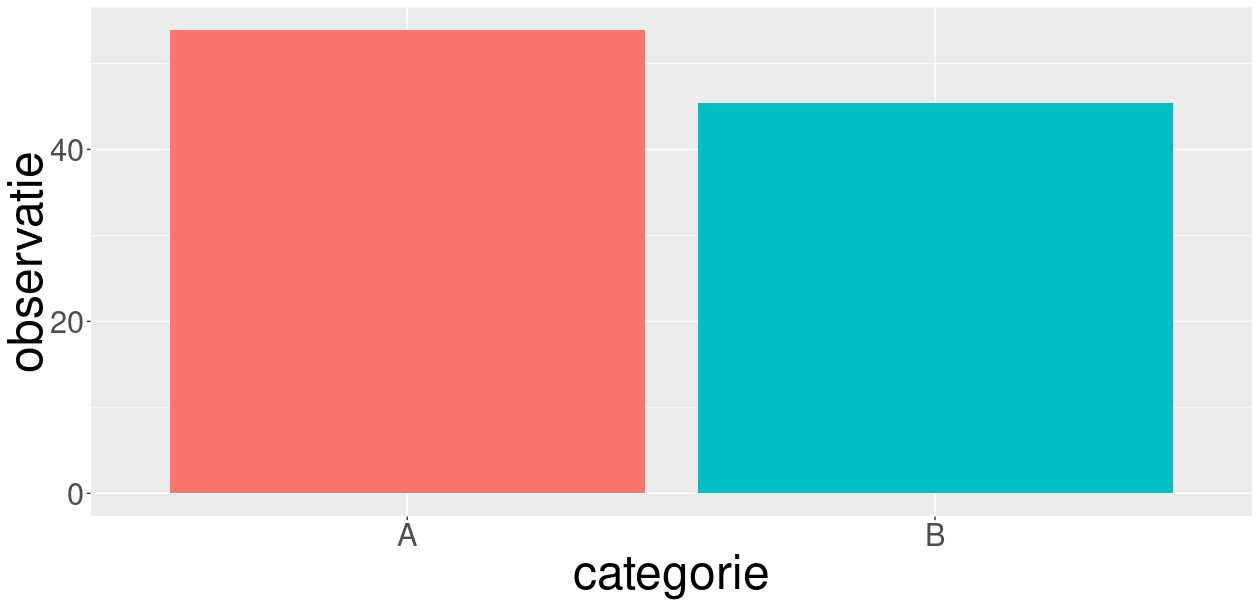
\includegraphics[width=\textwidth]{voorbeelden/barplot.png}
    \caption{Staafdiagram van gemiddelden. Dit is onvoldoende om een conclusie te trekken}
    \label{fig:barplot}
  \end{subfigure}
  \begin{subfigure}{.5\textwidth}
    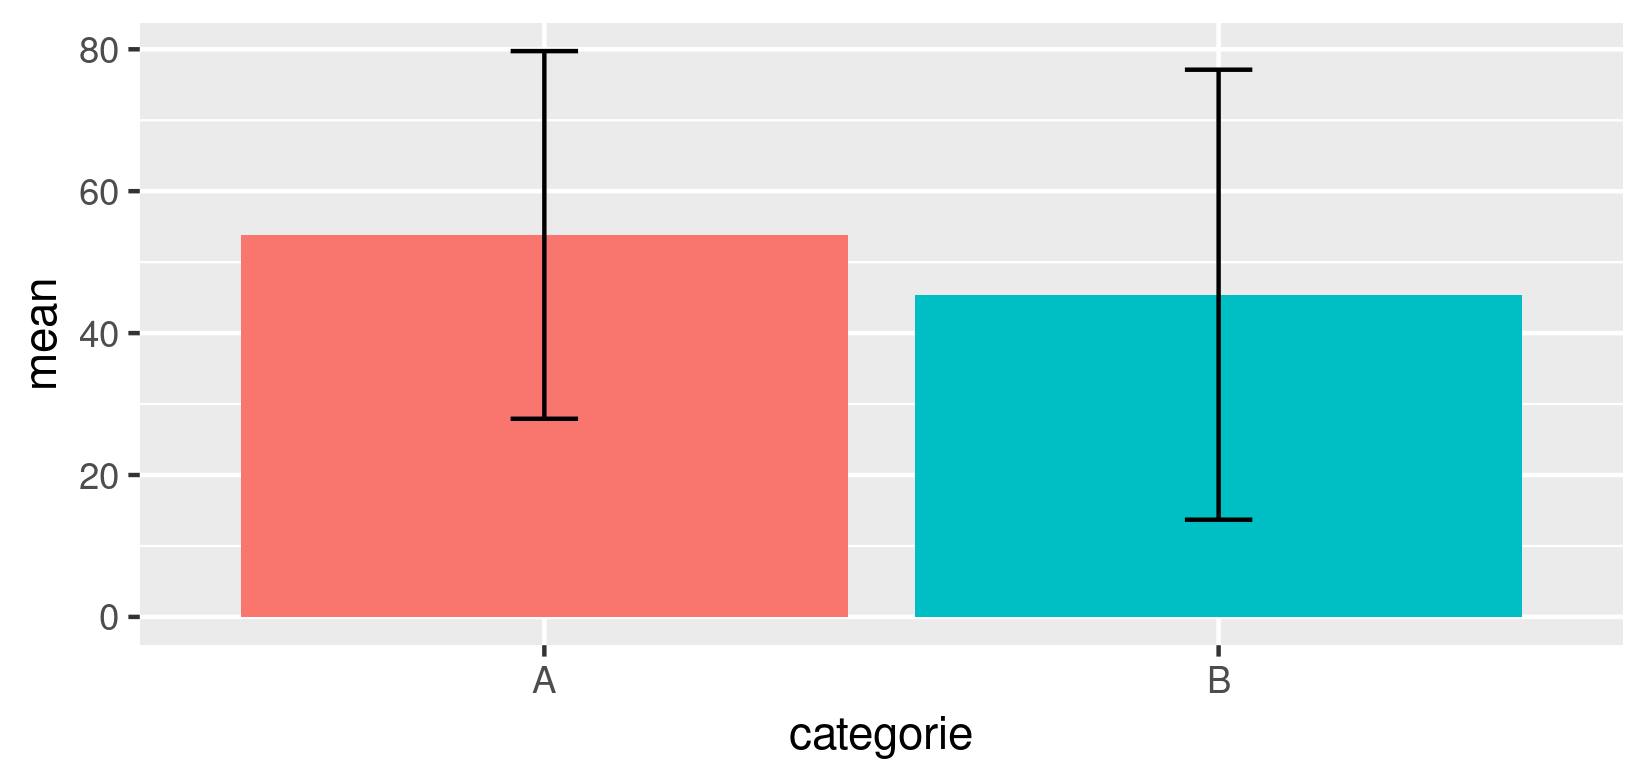
\includegraphics[width=\textwidth]{voorbeelden/barplot-errorbars.png}
    \caption{Staafdiagram met \textit{error bars} die de grootte van de steekproefstandaardafwijking voorstellen. Door de grote spreiding is het verschil tussen beide categorieën ineens veel minder uitgesproken.}
    \label{fig:barplot-errorbars}
  \end{subfigure}
  
  \begin{subfigure}{.5\textwidth}
    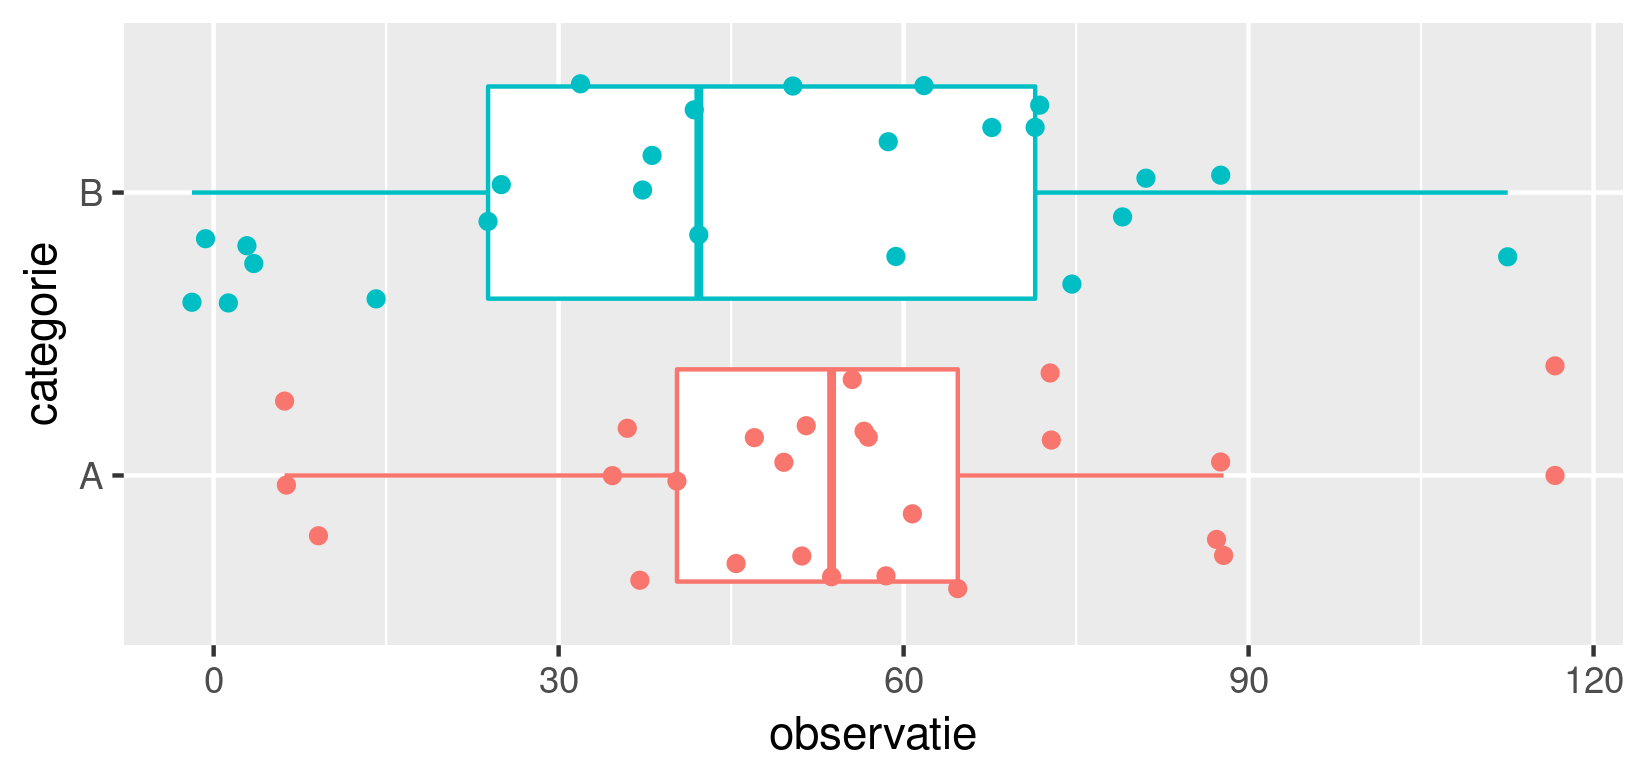
\includegraphics[width=\textwidth]{voorbeelden/boxplot-jitter.png}
    \caption{Boxplot met individuele observaties weergegeven als punten. Hiermee is de spreiding van de data nog duidelijker.}
    \label{fig:boxplot-jitter}
  \end{subfigure}
  \begin{subfigure}{.5\textwidth}
    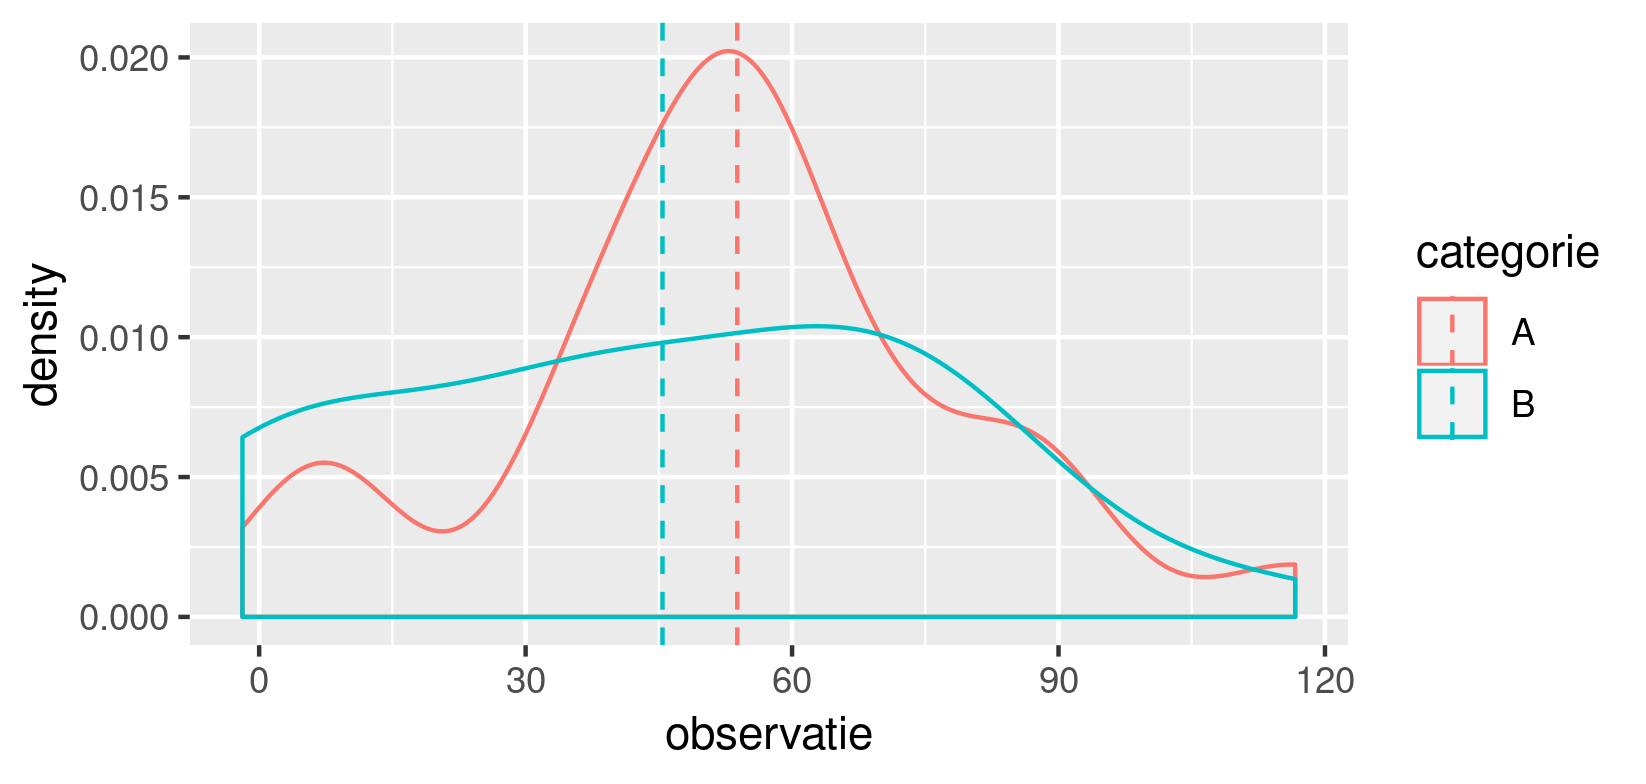
\includegraphics[width=\textwidth]{voorbeelden/density-plot.png}
    \caption{Kansdichtheid met steekproefgemiddelden aangeduid als een verticale stippellijn. Hier wordt duidelijk dat de resultaten van het experiment niet normaal verdeeld zijn. Dat maakt dat een staafdiagram met error bars eigenlijk niet geschikt is voor deze data.}
    \label{fig:density-plot}
  \end{subfigure}
  
  \caption[Visualiseren van cijfergegevens]{Verschillende manieren om dezelfde data te visualiseren.}
\end{figure}

